\chapter{Verwandte Arbeiten}\label{cha:verwandteArbeiten}
Im folgenden Kapitel gehen wir auf verschiedene Hintergründe und verwandten Arbeiten ein. 
Zur besseren Einordnung beginnen wir mit einer Einführung des Interaktionsraumes im Fahrzeug und geben einen kurzen Überblick zu den Bereichen Design und Evaluation von Informationssystemen im Auto.

Anschließend werden drei Modelle zu Vorhersage von Interaktionszeiten vorgestellt. 
Dabei gehen wir besonders auf das Konzept des Keystroke-Level Modell und Erweiterungen ein und stellen die verwandten Arbeite in diesem Bereich vor. 

Zuletzt befassen wir uns mit multimodalen Interaktionen, sowie mit multimodaler Interaktion im automobilen Kontext.   

\section{Interaktionsraum beim Fahren}
In heutigen Fahrzeugen wird dem Fahrer eine Vielzahl von Informationen und Entertainment Funktionen angeboten
Diese stellen einen multifunktionalen Raum für den Fahrer dar \citep{Kern:2009}. 
Ausgestattet mit Medienfunktionen, Navigationssystemen, die mittels GPS ortsbezogene Funktionen bieten (zum Beispiel "`finde die nächste Raststätte"'), Kommunikationssystemen und dem angeschlossenen Smartphone, bieten Fahrzeuge auch einen vernetzten Interaktionsbereich.

Beim Fahren werden drei verschiedene Aufgabenbereiche unterschieden \citep{geiser1985man}. 
\begin{figure}
	\centering
	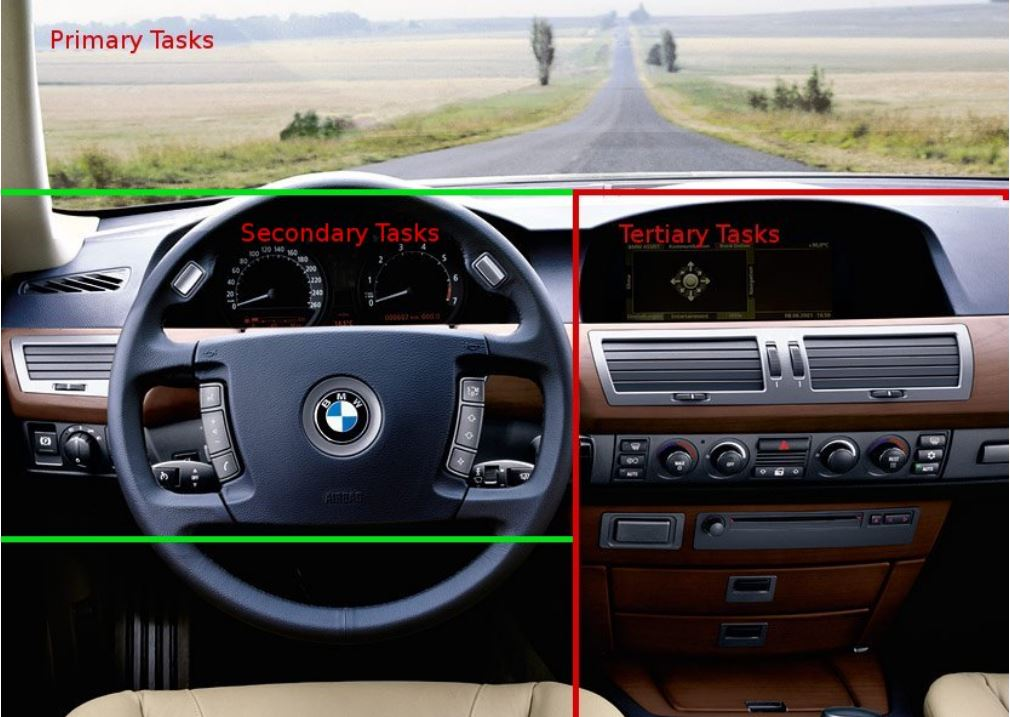
\includegraphics[width=0.5\textwidth]{img/Fahrbereiche_Tonnis.JPG}
	\caption{Aufteilung der Bereiche von primären, sekundären und tertiären Aufgaben. Bild entnommen aus \citet{Tonnis:2006}}
	\label{fig:Fahrbereiche_Tonnis}
\end{figure}
Die wichtigste Aufgabe des Fahrers ist das Fahren an sich, also die sichere Fortbewegung zum Ziel. 
Diese Aufgabe wird als primäre Aufgabe (Primary Task) kategorisiert und beinhaltet das Fahren, Bremsen, Spur halten und Lenken. 
Sekundäre Aufgaben (Secondary Tasks) bilden eine weitere Kategorie.
Sie unterstützen mit Aktionen und Reaktionen die primäre Aufgabe und die Sicherheit des Fahrens.
Hierzu gehören zum Beispiel das Blinken oder das Einschalten des Lichts bei Dunkelheit. 
Die letzte Kategorie sind die tertiären Aufgaben (Tertiary Tasks).
Sie beinhalten alle Aufgaben, die unabhängig vom Fahren gemacht werden können, wie zum Beispiel die Bedienung von Komfortfunktionen, Kommunikationsfunktionen oder Entertainmentfunktionen, aber auch Interaktionen mit dem Beifahrer \citep{geiser1985man}, \citep{Kern:2009}. 
Diese dritte Kategorie ist ein wesentlicher Bestandteil der Ablenkungen des Fahrers und führt oft zu Fahrfehlern oder sogar Unfällen \citep{neale2005overview}, \citep{rumar1988vehicle}. 

\subsection[Design von IVIS]{Design von Informationssystemen im Auto}
Beim Design von Informationssystemen im Auto (IVIS) ist es wichtig im Kopf zu behalten, wer unsere Nutzer sind.
Das Alter von Autofahrern kann sich von 16 bis über 90 Jahren erstreckt. 
In der Gruppe der 21-75 jährigen haben über 80\% einen Füherschein \citep{Green_2002}.
Unsere Nutzergruppe spiegelt also einer sehr große Altersspanne wieder. 
Es ist zu erwarten, dass die verschiedenen Altersklassen mit unterschiedlicher Performanz Aufgaben verrichten \citep{Green_2002}. 
Um Informationssysteme möglichst für jeden leicht verständlich zu gestalten, gibt es bereits viele Richtlinien, Prinzipien und Standards.
Beim Design von Informationssystemen im Auto beachtet sollten diese beachtet werden (siehe unter anderem Alliance of Automobile Manufacturers (AAM) \citep{driver2006statement}, National Highway Traffic Safety Administration (NHTSA) \citep{national2012visual}, European Statement of Principles (ESoP) \citep{national2012recommandationl}, ISO, Society of Automotive Engineers (SAE) oder DIN).
\citet{Green:2012:USI:2390256.2390258} hat dazu auch einige der Standards verglichen und zusammengefasst.

\subsection[Evaluation von IVIS]{Evaluation von Informationssystemen im Auto}
Informationssysteme im Auto können das Fahrverhalten negativ durch Ablenkung beeinflussen. 
Deshalb ist es wichtig solche Systeme zu evaluieren, um den Effekt der Ablenkung, die mentalen Belastung und die Interaktionsdauer zu messen. 
Es gibt verschiedene Methoden um ein neues System oder einen neuen Prototypen zu testen. 
\citet{burnett2008designing} zeigt in seiner Abbildung \ref{fig:Evaluation_of_in_car_computing_devices_Burnett2008} die verschiedenen Evaluationstypen von einer realen Feldstudie auf der Straße bis hin zu Laborstudien. 
\begin{figure}
	\centering
		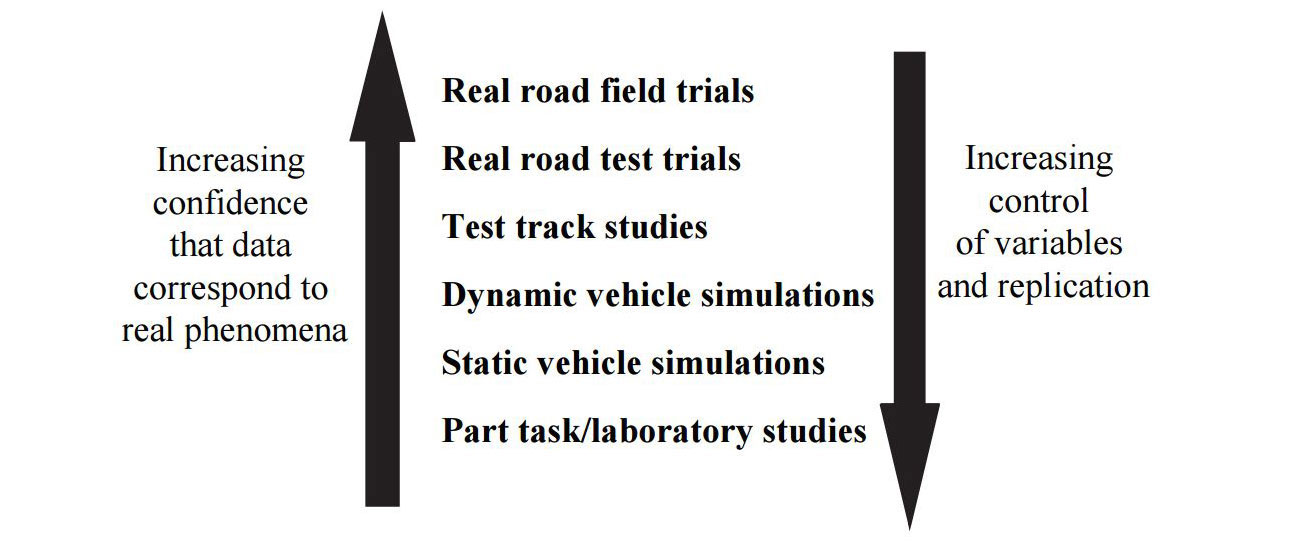
\includegraphics[width=1\textwidth]{img/Evaluation_of_in_car_computing_devices_Burnett2008.jpg}
	\caption[Evaluierungstypen und ihre Abhängigkeit zu Validität und deren Kontrollierbarkeit]{
Evaluierungstypen und ihre Abhängigkeit zur Validität und deren Kontrollierbarkeit. 
Bei realen Feldstudien verhalten sich Fahrer sehr natürlich, jedoch ist es schwer die Beeinflussung von Variablen zu kontrollieren. 
Im Gegensatz dazu können in Laborstudien die Variablen genau kontrolliert werden, jedoch ist das Fahrverhalten konstruiert und entspricht nicht mehr dem natürlichen Verhalten. 
Idee und Bild aus \citet{burnett2008designing}}
	\label{fig:Evaluation_of_in_car_computing_devices_Burnett2008}
\end{figure}

In realen Feldstudien zur Untersuchung des Fahrverhaltens werden die Fahrzeuge zur Erhebung gewünschter Werte instrumentiert und über einen Zeitraum beobachtet. 
Mit dieser Methode können unter realistischen Bedingungen Daten erhoben werden. 
Allerdings können Variablen wie das Wetter oder die Verkehrslage nicht beeinflusst werden. 
In einer High Fidelity Fahrsimulation können äußere Einflüsse wie die Verkehrslage kontrolliert werden, jedoch nimmt hier bereits das natürliche Fahrverhalten ab, da sich der Fahrer offensichtlich in einer Studie befindet und sich möglicherweise anders verhält. 
Außerdem sind die Kosten und der Aufwand einer solchen Studie sehr hoch. 
Eine Low Fidelity Fahrsimulation ist einfacher umzusetzen, jedoch nimmt das realistische Fahrverhalten weiter ab. 
Die Validität der Daten ist bei realen Feldstudien am besten und nimmt bis zu den Laborstudien immer mehr ab. 
Umgekehrt ist die Kontrolle von Variablen und deren Wiederholbarkeit bei Laborstudien am besten und bei realen Feldstudien am unkontrollierbarsten.

Bei der Wahl einer Evaluierungsmethode sollte die Abwägung zwischen Validität der Daten und die Kontrollierbarkeit der Variablen bewusst getroffen werden.

Wir stellen im Folgenden fünf Varianten vor, mit denen IVIS bereits evaluiert wurden. Die 15-Sekunden Regel, der NASA Task Load Index (NASA TLX), der Driving Activity Load Index (DALI), die Okklusions Methode und der Lane-Change Test. 
Diese Varianten können in einem stehenden Fahrzeug getestet werden. 

\subsubsection{15-Sekunden Regel}
Die Länge einer sekundären oder tertiären Aufgabe steht in Korrelation mit dem Unfallrisiko. Da es einfacher ist die Gesamtdauer einer Aufgabe (Total Task Time) zu bestimmen, ist die 15 Sekundenregel eine vereinfachte Annahme, dass eine Aufgabe in einem stehenden Auto nicht länger als 15 Sekunden dauern soll \citep{green199915}. 
Diese Regel ist die Grundlage eines vom Society of Automotive Engineers (SAE) vorgeschlagenen Standards \citep{green1999sae}. 
\citet{green1999sae} definiert die Dauer in einem stehenden Auto oder einer Attrappe gemessen, in dem der Proband nur die gewünschte Aufgabe ausführt. TODO(Satz kapier ich nich)
Das entspricht der Total Task Time, die wir in unserer Studie ebenfalls verwenden werden.

\subsubsection{NASA TLX}
\citet{hart1988development} entwickelte den NASA Task Load Index, dessen Verfahren die mentale Belastung in 6 Dimensionen misst. 
Dafür verwenden wir die deutsche Übersetzung des NASA TLX. 
Die Beanspruchungen werden unterschieden in: 
\begin{enumerate}
	\item \textbf{Geistige Anforderungen:} Wie viel geistige Anstrengung war bei der Informationsaufnahme und -verarbeitung erforderlich (zum Beispiel Denken, Entscheiden, Rechnen, Erinnern, Hinsehen, Suchen)? 
War die Aufgabe leicht oder anspruchsvoll, einfach oder komplex, erforderte sie hohe Genauigkeit oder war sie fehlertolerant?
	\item \textbf{Körperliche Anforderungen:} Wie viel körperliche Aktivität war erforderlich (zum Beispiel Ziehen, Drücken, Drehen, Steuern, Aktivieren)? 
	War die Aufgabe leicht oder schwer, einfach oder anstrengend, erholsam oder mühselig?
	\item \textbf{Zeitliche Anforderungen:} Wie viel Zeitdruck wurde hinsichtlich der Häufigkeit oder dem Takt, mit dem Aufgaben oder Aufgabenelemente auftraten, empfunden? War die Abfolge langsam und geruhsam oder schnell und hektisch?
	\item \textbf{Leistung:} Wie erfolgreich wurde die vom Versuchsleiter (oder dem Probanten selbst) gesetzten Ziele erreicht? Wie zufrieden war der Probant mit seiner Leistung bei der Verfolgung dieser Ziele?
	\item \textbf{Anstrengung:} Wie hart musste Der Probant arbeiten, um den Grad an Aufgabenerfüllung zu erreichen?
	\item \textbf{Frustration:} Wie unsicher, entmutigt, irritiert, gestresst und verärgert (im Gegensatz zu sicher, bestätigt, entspannt und zufrieden mit sich selbst) fühlte sich der Probant während der Aufgabe?
\end{enumerate}
Für jede dieser Beanspruchungen wird ein Wert zwischen 1 (gering) und 20 (hoch) abgefragt. 
Anschließend werden im zweiten Teil noch die 6 Beanspruchungen verglichen. 
Es werden alle Beanspruchungen gegenüber gestellt und der Proband muss sich immer für die Beanspruchung entscheiden, die aus seiner Sicht wichtiger ist. 
Somit wird eine Gewichtung ermittelt, um den Grad der Belastung genauer bestimmen zu können. 
Diese Bestimmung der Beanspruchung mit dem NASA TLX ist weitverbreitet und wird regelmäßig in der Forschung verwendet \citep{hart2006nasa}. 
Teilweise wird die kurzen Version (ohne die Gewichtung durch den zweiten Teil) verwendet. 

\subsubsection{DALI}
Sehr ähnlich zu dem NASA TLX ist der DALI, der sich jedoch auf den automobilen Kontext bezieht und den Beanspruchungswert mit angepasster Gewichtung berechnet. 
Der DALI evaluiert die subjektive mentale Belastung eines Fahrers während der Fahrt \citep{pauzie2008method}, mit oder ohne die Unterstützung eines Informationssystems. 
Eine weitere Technik zur subjektiven Einschätzung der Belastung ist die "`Subjective Workload Assessment Technique"' (SWAT), siehe \citep{reid1982subjective}.

\subsubsection{Okklusions Methode}
Hierbei wird die visuelle Belastung von IVIS für die sekundären Aufgaben gemessen. 
Diese Verschluss Methode soll die Abwendung des Blickes simulieren, die zwischen der Hauptaufgabe dem Fahren und dem Blick zum IVIS passiert. 
Die Hauptidee besteht darin die Sicht, durch Abdeckung, abwechselnd für 1,5 Sekunden zu verhindern und anschließend für 1,5 Sekunden zu ermöglichen. 
Heutzutage gibt es spezielle Brillen mit denen diese Methode durchgeführt werden kann \citep{pettitt2006assessment}.

\subsubsection{Lane Change Test (LCT)}
Dieser Test wurde in Kooperation von DaimlerChrysler und BMW von \citet{mattes2003lane} entwickelt. 
Er misst die Performanz von Doppelaufgaben. 
Der Proband muss eine simulierte Fahraufgabe lösen. 
Diese ist in abstrakter Weise dargestellt und es muss auf einer dreispurigen Autobahn zwischen den Spuren gewechselt werden. 
Wann gewechselt werden muss wird mit Schildern angezeigt und es werden hieraus verschiedenen Zeiten gemessen (wie lange dauert ein Wechsel, wurde jedes mal richtig gewechselt). 
Diese Fahraufgabe löst der Proband zuerst ohne sekundäre Aufgabe.
Dies wird als Referenzwert verwendet. 
Anschließend soll der Proband sowohl die Fahraufgabe bewerkstelligen, als auch das zu Testende IVIS. 
Natürlich hat dabei die Fahraufgabe die höhere Priorität.  
Am Ende können die Zeiten von reiner Fahraufgabe und Fahraufgabe mit IVIS verglichen werden. 
Diese Methode kommt dem natürlichen Fahrverhalten deutlich näher, als der 15- Sekunden Regel und der Okklusion Methode.

\section[Vorhersagemodelle]{Modelle zur Vorhersage von Interaktionszeiten}
Zur Vorhersage von Bedien- oder Interaktionszeiten gibt es verschiedene Ansätze und Modelle. 
In den nächsten Unterkapiteln stellen wir drei Varianten vor. 
Dabei gehen wir vor allem auf das Keystroke-Level Modell und dessen Erweiterungen ein. 

\subsection[Fitts` Law]{Fitts` Law}
Der Psychologe Paul Fitts entwickelte 1954 ein Gesetz, dass die Zeit berechnet, die eine eindimensionale Bewegung einer Strecke zu einem Ziel einer bestimmten Größe benötigt \citep{fitts1954information}. 
\begin{figure}
	\centering
		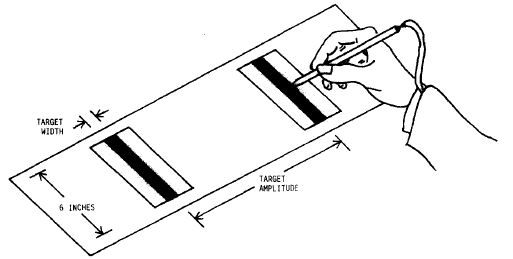
\includegraphics[width=0.7\textwidth]{img/FittsLaw.JPG}
	\caption[Orginaler Aufbau des Versuchs zur Erstellung von Fitts` Law]{Orginaler Aufbau des Versuchs zur Erstellung von Fitts` Law. 
	Die schraffierten Bereiche sollten abwechselnd mit dem Stift getroffen werden, ohne den Bereich zu überschreiten \citep{fitts1954information}. }
	\label{fig:FittsLaw}
\end{figure}

Dieses Gesetz bekam im laufe der Zeit den Namen Fitts` Law und wurde in der Mensch-Maschine Interaktion oft verwendet. 
Die Formel hat ihren Ursprung bei MacKenzie \citep{MacKenzie:1992} und berechnet sich wie folgt:
\[
\text{MT} = a+b * log_2 (\frac{D}{W}+1)
\]
Wobei MT der Bewegungszeit (movement time) entspricht, $a$ und $b$ Konstanten sind, $D$ die Distanz des Startpunkts bis zur Mitte des Zielobjekts ist und $W$ die Breite des Objekts darstellt, die entlang der Bewegungsrichtung gemessen wird. 
Aus Fitts` Law können wir entnehmen, dass Distanz und Bewegungszeit positiv korreliert sind , das heißt mit größer werdender Distanz sich die Zeit verlängert.
Zeit und Größe des Zielobjekt sind dagegen negativ korreliert, das heißt mit größer werdendem Zielobject verkürzt sich die Zeit.
Bei Designentscheidungen kann mit Fitts` Law die schnellere Variante berechnet werden. 
Zum Beispiel bei zwei Konzepten für eine Interface mit unterschiedlich großen Buttons, die unterschiedlich positioniert sind. 

\subsection[GOMS]{GOMS}
Ein weiteres Modell zur Vorhersage von Interaktionszeiten auf einem Bildschirm mit Eingabe durch Tastatur und Maus ist GOMS (Goal, Operator, Method und Selection Rules). 
Bei GOMS wird das Ziel durch ein Set von Methoden und dessen Operatoren erreicht und durch die Selektionsregeln werden die entsprechenden Methoden gewählt \citep{card1983psychology}.
Interaktionsschritte können somit von oben nach unten (top-down) strukturiert und dargestellt werden \citep{butz2014mensch}. 

\subsection{Keystroke-Level Modell (KLM)}
Das Keystroke-Level Modell ist eine vereinfachte Variante von GOMS und baut sich umgekehrt von unten nach oben (bottom-up) auf. 
Das ursprüngliche Keystroke-Level Modell (KLM) wurde von \citet{Card_1980} für Desktopanwendungen mit Tastatur entwickelt. 
Mit dem Keystroke-Level Modell kann die Zeit vorhergesagt werden, die ein Experte benötigt, um eine bestimmte Aufgabe zu lösen. 
Um diese Zeit vorhersagen zu können wird die Aufgabe in ihre Einzelschritte den Operatoren unterteilt und deren Zeiten aufsummiert. 
Diese resultierende Zeit entspricht der "`Total Task Time"', also die Zeit, die benötigt wird bis ein Nutzer die gesamte Aufgabe vollendet hat. 
Das Set von Operatoren besteht aus einen mentalen Operator \textbf{M} und vier physischen Operatoren. 
Der mentale Operator entspricht einer Vorbereitungszeit, die ein Nutzer vor oder zwischen Operatoren benötigt.
\begin{figure}
	\centering
		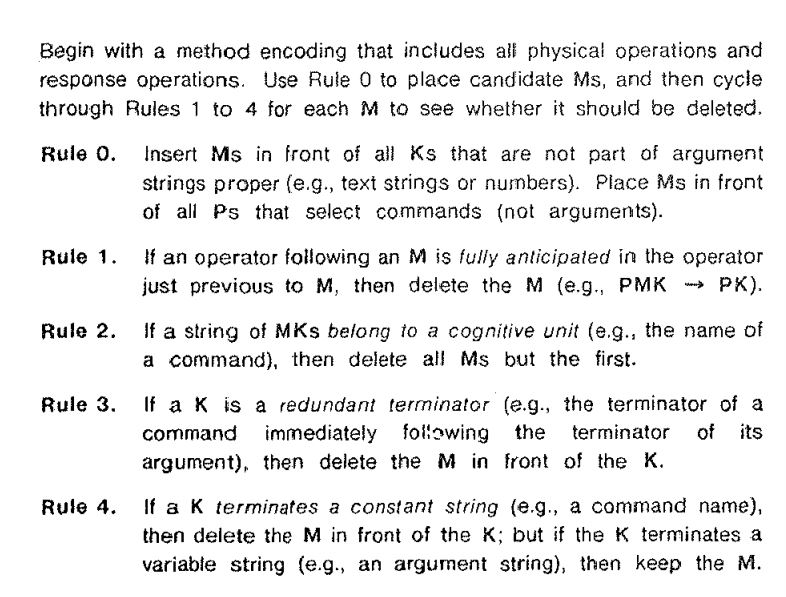
\includegraphics[width=0.7\textwidth]{img/KLM_Mental_Operator_Rules.JPG}
	\caption{Plazierungsregeln des mentalen Operators}
	\label{fig:KLM_OPeratoren}
\end{figure}
Um das Keystroke-Level-Model richtig anzuwenden werden noch Regeln vorgegeben, um den mentalen Operator \textbf{M} richtig zu platzieren. 
Es gibt 5 verschiedene Regeln mit deren Hilfe die Berechnung einer Aufgabe alle benötigten physischen und mentalen Operatoren vorgibt. 
Die 4 physischen Operatoren sind:
\begin{itemize}
	\item \textbf{K (Keystroke)}: Tastenklick
	\item \textbf{P (Pointing)}: Maus zu einem Zielort verschieben
	\item \textbf{D (Drawing)}: ein Set von geraden Linien mit der Maus malen
	\item \textbf{H (Homing)}: der Wechsel zwischen Maus und Tastatur
\end{itemize}
Außerdem gibt es noch den Operator R(t), der die Antwortdauer des Systems darstellt. 

Es wird grundsätzlich bei den Zeiten von Experten ausgegangen, die keine Fehler machen, jedoch werden beim Tippen von Texten (Operator K) 7 Kategorien unterschieden. 
Diese Zeiten haben eine Spanne vom besten Tipper bis zum schlechtesten Tipper, siehe \fref{fig:KLM_OPeratoren}.
\begin{figure}
	\centering
		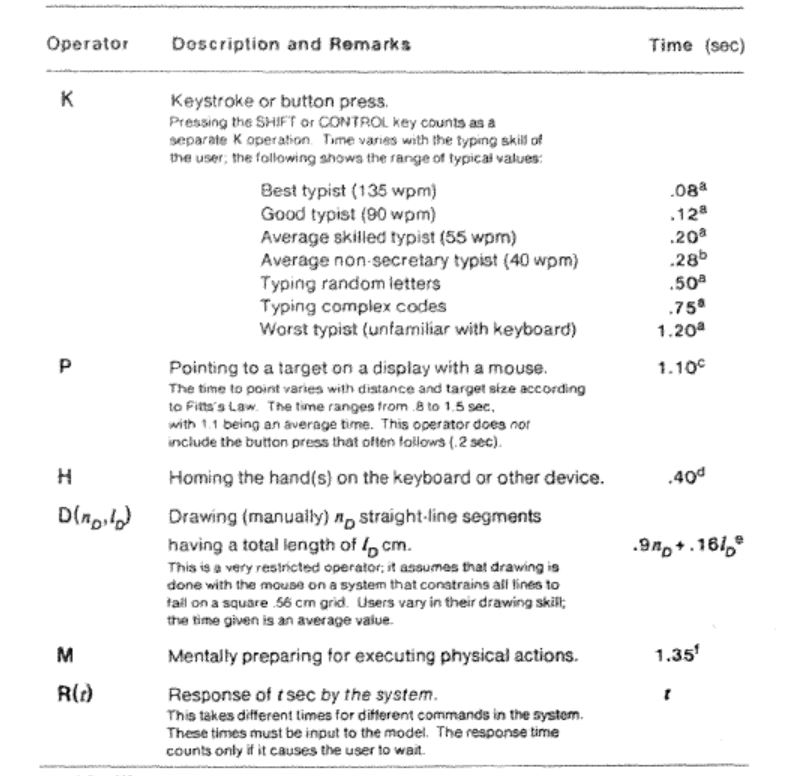
\includegraphics[width=0.7\textwidth]{img/KLM_OPeratoren.JPG}
	\caption{Orginale Tabelle der Operatoren von \citet{Card_1980}}
	\label{fig:KLM_OPeratoren}
\end{figure}

Dieses Modell ermöglicht in einem sehr frühen Stadium der Entwicklungsphase, bereits vor der Implementation, vorherzusagen wie lange Experten für bestimmte Aufgaben benötigen. 
Dieses Modell wurde bereits in vielen Studien angewendet und immer wieder auf Weiterentwicklungen angepasst.
Um bei beliebigen Interfaces schnell und ohne Fehler das KLM zu erzeugen entwickelten \citet{John_2004} ein Tool (später auch CogTool genannt), das von neuen Interfaces das KLM automatisch generiert und somit das Testen von neuen Interfaces noch einfacher macht.

Mit dem Fortschritt der Technik kommen ständig neue Anwendungen mit neuen Modalitäten auf den Markt, die implementiert und getestet werden müssen. 
Deshalb wurde im Laufe der Zeit das KLM immer weiter an aktuelle Geräte und Interfacekonzepte angepasst. 
In den folgenden Abschnitten geben wir eine Zusammenfassung der Erweiterungen des Keystroke-Level Modell.
\subsection[KLM für tragbare Geräte]{Erweiterung des KLM für tragbare Geräte}
\citet{Luo_2005} haben das Modell für tragbare Geräte mit Stiftnutzung statt der Tastatur erweitert beziehungsweise auf diesen Kontext angepasst. 
Die Modelle wurden mit Hilfe der für KLM entwickelten Software CogTool generiert \citep{John_2004}. 
Die vorhergesagten und die gemessenen Zeiten betrugen nur einen Vorhersagefehler von weniger als 8\%.
\citep{Holleis_2007} und \citep{Li_2010} ergänzen das KLM für die Handynutzung. 
\citeauthor{Li_2010} geht dabei mehr auf stiftbasierte Operatoren ein und \citet{Holleis_2007} betrachten mehr die haptischen Tasten auf Handys und führt allgemeinere Operatoren hinzu. 
\citet{Holleis_2007} erweitert das Keystroke-Level Modell unter anderem mit 7 neuen Operatoren, um die Dauer von  fortgeschrittenen Interaktionen auf Handys vorhersagen zu können. 
Diese neuen Operatoren sind:
\begin{itemize}
	\item \textbf{Macro Attencion Shift ($S_\text{Macro}$):} Wechsel zwischen dem Handy und der realen Welt.
	\item \textbf{Micro Attention Shift ($S_\text{Micro}$):} Wechsel zwischen Display, Tastatur und dem Hotkeybereich.
	\item \textbf{Distraction (X):} Ein Ablenkungsfaktor wird mit den Operationen multipliziert.
	\item \textbf{Action (A(t)):} Aktionen, die nicht in Operatoren unterteilt werden können.
	\item \textbf{Gesture (G):} Gestenerkennung wie zum Beispiel das Handy drehen oder Zahlen in die Luft malen.
	\item \textbf{Fingermovement (F):} Fingerbewegung von einer Position zu einer anderen.
	\item \textbf{Initial Act (I):} Zeit um zum Beispiel das Handy aus der Tasche zu holen.
\end{itemize}
Die Operatoren K, P und H des orginalen KLM werden etwas angepasst, M bleibt gleich und D wird nicht benötigt.
 
\citet{Li_2010} kombinieren das KLM mit einem neuen Konzept von Operator Blöcken. 
Ein Operator Block enthält eine Sequenz von Operatoren, die häufig als Einheit in Aktionen vorkommen. 
Dem originalen KLM werden neun physische Operatoren hinzugefügt und fünf mentale Operatoren, wovon vier für die Stiftnutzung angelegt sind. 
Teils entsprechen die physischen Operatoren denen von \citet{Holleis_2007} und teils werden deren Operatoren wieder verworfen. 

\subsection[KLM für Touch]{Erweiterung des KLM für Toucheingaben}
Nachdem bei mobilen Geräten wie Smartphones oder Tablets mehr und mehr die Stiftnutzung verschwindet und eingebaute Touchscreens verwendet werden wurde auch in diesem Bereich das KLM erweitert. 
\citet{Abdulin_2011} untersuchte das KLM für direkten Touch auf 7-17 Zoll großen Tablets. 
Die KLMs von drei verschiedenen Interfaces wurden mit dem CogTool generiert und mit Studienzeiten verglichen. 

Ebenfalls auf Touchscreens fokussieren sich \citet{ElBatran_2014} und \citet{Rice_2014}. \citet{ElBatran_2014} gewinnt in drei Studien Zeiten für drei Touch-Operatoren: Swipe, Zoom und Tap. \citet{Rice_2014} erstellen ein neues Set von Operatoren, dem Touch-Level Modell, zusammen. 
Dafür lassen sie die ursprünglichen Operatoren K, H, M und R(t) unverändert. 
Die Operatoren X und I werden von \citet{Holleis_2007} übernommen und acht weitere Operatoren hinzugefügt: 
\begin{itemize}
	\item \textbf{Gesture (G)}: Geste mit 1, 2 oder mehreren Fingern
	\item \textbf{Pinch (P)}: 2-Fingergeste, wobei die Finger am Ende geschlossen sind
	\item \textbf{Zoom (Z)}: 2-Fingergeste, wobei die Finger am Anfang geschlossen sind
	\item \textbf{Tap (T)}: Finger-Tap
	\item \textbf{Swipe (S)}: Finger auf dem Touchscreen bewegt sich in horizontaler oder vertikaler Richtung
	\item \textbf{Tilt (L(d))}: Neigung oder Rotation des ganzen Geräts um d Grad
	\item \textbf{Rotate (O(d))}: 2-Fingergeste mit der auf dem Screen etwas um d Grad rotiert wird
	\item \textbf{Drag (D))}: 1-Fingergeste mit der meist ein Objekt von einer Position zu einer anderen gebracht wird
\end{itemize}
Das Touch-Level Modell soll in zukünftigen Studien noch verifiziert und evaluiert werden.
\subsection[KLM im automobilen Kontext]{Erweiterung des KLM im automobilen Kontext}
Die Infotainmentsysteme in Autos werden immer komplexer und auch hier ist es wichtig für Designer in einem frühen Stadium Interfaces testen zu können. 
Es gibt im Auto nicht nur ein Gerät das betrachtet werden kann, sondern mehrere Bereiche mit verschiedensten Bedienelementen. 
Diese Bedienelemente können ursprüngliche haptische Knöpfe und Schalter sein, aber auch Touchdisplays und mögliche Einrichtungen für Sprach- oder Gestensteuerungen. 

\citet{Pettitt_2007} befassen sich 2007 mit diesem Thema und erweitern das KLM für Informationssysteme im Auto, mit Hinzunahme der Occlusion Technik. 
Die Zeiten dieses KLM werden dann mit den Zeiten von einer Occlusion Studie verglichen. 
Sie verwenden die Operatoren von \citet{Card_1980} und der Operator $R_f$ (Reach far) wurde von \citet{Green_2002} adaptiert, genau wie der Operator (Reach near), dessen Zeit für die Bewegung innerhalb eines Systems mit Fitt's Law berechnet wird.

Ebenfalls im automobilen Kontext erweitert \citet{schneegass_2009} (siehe auch \citep{SchneegaB_2011}) das KLM und bezieht sich dabei im speziellen auf die Interaktionen von Autoradios. 
In dieser Studie werden vier Aufgaben in diesem Kontext mit insgesamt 78 Operatoren aufgezeichnet und deren Zeiten berechnet. 
Der interessanteste und für den automobilen Kontext neu hinzugefügte Operator ist der Turn (T) Operator. 
Dieser Operator wird für alle haptisch drehbaren Knöpfe verwendet und es wurden jeweils drei verschiedene Drehwinkel für Linksdrehungen (negativ) und Rechtsdrehungen (positiv) untersucht ($-180^\circ$, $-90^\circ$, $-45^\circ$, $45^\circ$, $90^\circ$, $180^\circ$). 
\begin{figure}[ht]
  \centering
  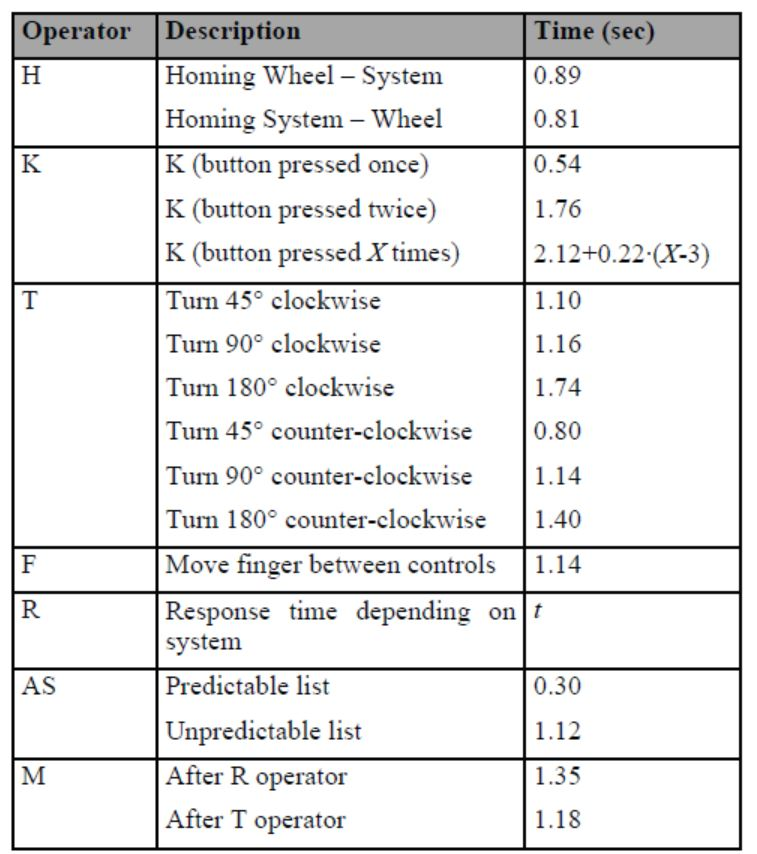
\includegraphics[width=0.7\textwidth]{img/Schneegass_KLM_Operator_Table.jpg}
  \caption[Tabelle der Operatorzeiten von Schneegaß]{Tabelle der Operatoren, deren Beschreibung und den dazugehörigen Zeiten.}
  \label{fig:Bild1}
\end{figure}

Schneegaß verweist darauf, dass die Berechnung der Zeiten für den Turn(T) Operator in Zukunft noch genauer untersucht werden sollte, indem zusätzlich unterschieden wird, ob in einen bestimmten Bereich gedreht oder ein bestimmter Winkel der Drehung verlangt wird. 
Die genauen Zeiten der einzelnen Operatoren können aus \fref{fig:Bild1} von \citet[Seite 75]{SchneegaB_2011} entnommen werden. 
Ein weiterer wichtiger Aspekt aus seinen Ergebnissen ist das Feedback der Teilnehmer dieser Studie. Es wurde angemerkt, dass die Aufgaben, mit bis zu sechs Unteraufgaben, zu lang waren. 
Somit war die kognitive Auslastung, sich diese Aufgaben zu merken, zu hoch. 
Außerdem reagierte das verwendetet System langsamer, als die Teilnehmer es von eigenen Autos gewohnt waren. 
Dieses Feedback versuchen wir in unserer Studie aufzugreifen, indem wir die Aufgaben möglichst kurz halten. 

\section[Multimodale Interaktion]{Multimodale Interaktion}
Multimodale Interaktion ist für Menschen etwas ganz natürliches, das unbewusst bei den meisten Kommunikationen zwischen Menschen gemacht wird. 
Zwei Leute unterhalten sich zum Beispiel und nebenbei zeigt einer zusätzlich auf einen Gegenstand, schauen in eine Richtung und kombinieren all diese zusätzlichen Informationen, die das gesamte Gespräch bereichern und erleichtern. 
Um unsere Außenwelt besser verstehen zu können schauen, hören, tasten und riechen wir zugleich \citep{sharma1998toward}. 
Um auch Interaktionen zwischen Mensch und Maschine intuitiver und natürlicher für zu gestalten könnte das Hinzufügen zusätzlicher Modalitäten eine große Bereicherung sein.

Multimodale Systeme können durch mehrere Kommunikationskanäle bedient werden. 
Die Mensch Maschine Interaktion geschieht zwischen den Aktoren und Sensoren des Menschen, siehe Grafik \ref{fig:Multimodalitaet}von \citep{neuss_2001}.
\begin{figure}
	\centering
		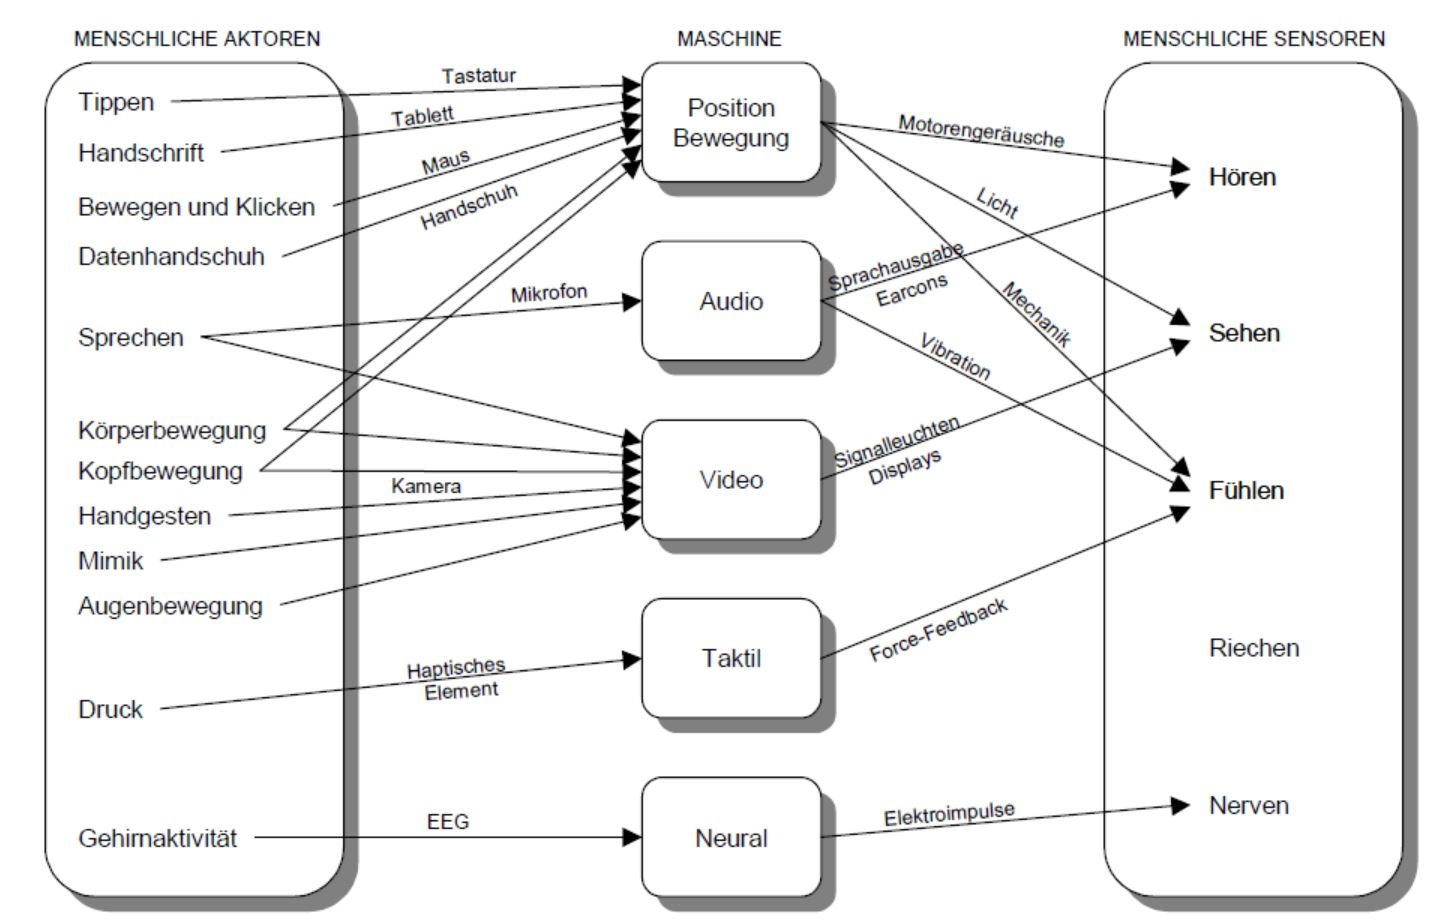
\includegraphics[width=1\textwidth]{img/Multimodalitaet.JPG}
	\caption[multimodale Kommunikationskanäle]{Die Abbildung von \citep{neuss_2001} beschreibt das Zusammenspiel von menschlichen Aktoren und Sensoren in Interaktion mit der Maschine. Das Modell ist abgeleitet von \citep{sharma1998toward}}
	\label{fig:Multimodalitaet}
\end{figure}
Doch wann kann ein Nutzer eine bestimmte Modalität verwenden oder zu einer anderen wechseln?
\citet{neuss_2001} differenziert in seiner Dissertation vier verschiedenen Ausprägungen der Multimodalität hinsichtlich der Eingabe.
\begin{itemize}
	\item \textbf{seriell-redundant:} Modalität kann beliebig gewechselt werden
	\item \textbf{seriell-exklusiv:} Modalität kann nur nach bestimmten Schritten gewechselt werden
	\item \textbf{parallel-ergänzend:} "`Simultan getätigte Eingaben mit verschiedenen Modalitäten ergänzen sich."'\citep{neuss_2001}
	\item \textbf{parallel-verifizierend:} "`Simultan getätigte Eingaben mit verschiedenen Modalitäten bestätigen sich gegenseitig"' \citep{neuss_2001}. Ein Beispiel wäre die Kombination aus Sprache und Lippenlesen.
\end{itemize}
Je nach Kontext wird die beste Variante gewählt. 
Alle Varianten, ob alleine oder in Kombination geben dem Nutzer mehr Freiheit das Ziel zu erreichen und erhöhen zudem die Effizienz \citep{neuss_2001}. 

Eine Herausforderung ist ein gutes Design von multimodalen Interfaces, sodass die Vorteile der Modalitäten genutzt werden können, aber auch die Bedienung den Nutzer unterstützt und nicht verwirrt. 
Dazu haben \citet{Reeves_2004} ein Regelwerk für das Design von multimodalen Interfaces erstellt. 
Deren Ziel ist es, dass in Zukunft Interaktionen natürlicher und intuitiver werden und die Robustheit durch redundante Informationen und Interaktionsmodalitäten gesteigert wird. 
Einige wichtige Aspekte sind hierbei das konsistente Design von Input und Output. 
Es soll zum Beispiel vermieden werden, dass redundante Informationen in verschiedenen Modalitäten präsentiert werden, wenn der Nutzer sich dabei auf zwei verschiedene Quellen konzentrieren muss. 
Der Output soll im gleichen Stil des Inputs gestalten werden. 
Außerdem ist es wichtig, dass ein multimodales Interface Design adaptiv und konsistent ist. 
Es soll ausreichend Feedback geben und eine gute Fehlerbehandlung lässt den Nutzer immer wissen, welche Fehler ihn zu einem Status gebracht haben. 

\section[Multimodale Interaktion im Auto]{Multimodale Interaktion im automobilen Kontext}
Multimodale Interaktion gibt es bereits in aktuellen Autos und dieser Bereich umfasst ein großes Feld an Möglichkeiten. 
Eine der bekanntesten Varianten multimodaler Interaktion im Auto, ist die Sprachbedienung mit der zum Beispiel Anrufe getätigt werden. 
Auch Touchdisplays von externen Navigationssystemen oder Informationssystemen werden immer häufiger verwendet. 
Einige interessante Forschungsansätze von multimodaler Interaktion im Auto stellen wir Ihnen vor.

\citet{Pieraccini_2004} entwickelte einen multimodalen Prototypen in einen Ford Model U. Dieser basiert auf ein sprach basiertes System, dass durch einen visuellen und haptischen Touch-Screen unterstützt wird. 
Diese Kombination soll Anfängern das Erlernen von Sprachbefehlen erleichtern, indem visuell Hilfen der Sprachbefehle auf dem Touch-Screen in jeder Ebene des Interfaces zu sehen sind. 
Für Experten ist die Nutzung von ganzen Sätzen möglich, ohne für jede Ebene ein eigenes Kommando verwenden zu müssen.
Nach jedem Sprachbefehl ist es möglich durch eine Touch-Geste den Modus zu Wechseln. 

Redundante Modalitäten haben viel Potenzial für das Design von modernen Interfaces, wie auch \citet{Muller_2011} in ihrem Artikel feststellten haben sie zwei signifikante Vorteile im Gebrauch von Autos: Es ist zu einem dem Fahrer möglich, die für ihn passenste Modalität je nach Situation zu wählen. 
Zum anderen können lange Interaktionen, von einer Modalität zur anderen, ohne Probleme gewechselt werden.

\citet{Bertoldi:2010} haben die Multimodalität in Fahrer Assistenz Systemen untersucht, mit dem Ergebnis, dass es in diesem Feld noch viel zu Forschen und zu verbessern gibt. 
Aber es hat das Potenzial die Sicherheit zu erhöhen, die Reaktionszeiten und die Eyes-off-the-road Zeit zu verkürzen und das Bewusstsein der Fahrersituation zu erhöhen. 

\citet{Doring:2011} erweiterten ein Lenkrad in der Mitte mit einer Multi-Touch Oberfläche und untersuchten deren Möglichkeiten für Touch-Gestensets. 
Die visuelle Ablenkung konnte durch Touchgesten reduziert werden. 

Eine ähnliche Idee hatten \citet{Pfleging_2012}. 
Sie entwickelten, unter Rücksichtnahme von guter Lernbarkeit, Sichtbarkeit, Granularität und der Möglichkeit Aktionen rückgängig zu machen, ein im Lenkrad integriertes multimodales System, das Sprache und Touchgesten kombiniert. 
Es stellte sich heraus, dass Sprache und Gesten langsamer sind als der Gebrauch von haptischen Buttons, jedoch bei ähnlicher Fahrperformanz die visuelle Anstrengung geringer ist. 
Ein Nachteil ist das nötige Erlernen und Erinnern von Sprachbefehlen und Gesten. 
In deren System wurde zuerst die Sprache verwendet um Objekte oder Funktionen direkt ohne hierarchische Struktur zu benennen und anschließend konnte mit einer Touchgeste deren Parameter justiert werden, siehe auch \citep{Pfleging_t_2011}. 
Bei den Sprachbefehlen wurden von 82,1\% die Benennung von Objekten bevorzugt. 
Bei den Touchgesten benutzten 78,1\% der Teilnehmer 1-Finger Touchgesten. 

\citet{stracke2014touch} untersuchte in seiner Bachelorarbeit Touch Interactionen auf der Mittelkonsole. 
In dieser Arbeit wurde Direct-Touch-Steuerung mit "`drei Formen positionsunabhängigen Wischgesten"' \cite[Seite 57]{stracke2014touch} dem Serial Swipe, dem Relative Swipe und einem Relative Swipe mit Multi-Touch verglichen. 
Mit der Direct-Touch-Variante konnte eine Verkürzung der Interaktionszeit festgestellt werden. 
Jedoch schnitt diese Variante bei der Fehlerrate schlechter als die anderen Varianten ab, allerdings konnte keine Signifikanz bewiesen werden. 
Sehr beliebt war die Direct-Touch-Steuerung zur Einstellung der Luftverteilung und für Ein-/Ausschaltoptionen. 

Im nächsten Schritt verschaffen wir uns in einem Workshop einen Überblick über multimodale Interaktionen im Auto.